\documentclass[10pt]{article}
\usepackage[letterpaper,margin=0.75in]{geometry}
\usepackage{graphicx,booktabs,caption,helvet,url}
\renewcommand{\familydefault}{\sfdefault}
\captionsetup{font=small,labelfont=bf}
\setlength{\parskip}{0.45em}\setlength{\parindent}{0pt}
\graphicspath{{../figs/}}
\pagestyle{empty}
\newcommand{\Itot}{I\textsubscript{tot}}
\newcommand{\Vbus}{V\textsubscript{bus}}

\begin{document}
{\Large\bfseries Drive-law noise reduction: fw v35 vs fw v37}\\[0.3em]
{\small Scale-car DC balancer board, Pi rosbag and SD-log analysis. Ricky Tan, 2026-11-06.}

\section*{1. Summary}
The fw v37 drive law lowers the drive-loop crossover from 2.76~Hz to 1.04~Hz. On the vehicle, it
reduces the once-per-revolution (1x) flywheel line to 0.25--0.28 of its fw v35 level on the bus
currents, the bus voltage and the FC share ratio. The design ratio is 0.29. Content above about
7~Hz is unchanged. A 1~kHz SD-card log shows that most of the remaining bus-voltage noise in the
Pi logs is high-frequency content folded by the 21~ms telemetry snapshot. Its largest source is
real bus current at the motor's 6x electrical frequency. The RT1987 ideal diodes and the boost
switching contribute little.

\section*{2. Data and method}
Two runs of the same SDP drive cycle are compared: \path{rosbag_sdp_2026-10-30_01-49-38}
(fw v35) and \path{rosbag_sdp_2026-11-05_20-09-52} (fw v37 rev 2). The share controller and
all other run-path code are identical in the two builds. Statistics use only samples with both
sources on the bus and \Itot{} $>$ 0.3~A. The analysis excludes $\pm$0.5~s around each H-20 purge
and $-$0.2/$+$1.0~s around each share-command step. Duplicate telemetry rows are removed, which
gives a sample rate of 47.62~Hz. The share is s = I\textsubscript{fc}/\Itot.

\section*{3. Results}
Table~1 gives the 1x amplitude from a tracked-phase lock-in at 1.8--2.9~m/s.

\begin{center}
\small
\begin{tabular}{lrrr}
\toprule
1x amplitude (peak) & fw v35 & fw v37 & Ratio \\
\midrule
\Itot & 213 mA & 54 mA & 0.25 \\
I\textsubscript{batt} & 187 mA & 47 mA & 0.25 \\
I\textsubscript{fc} & 34 mA & 9 mA & 0.27 \\
\Vbus & 14.2 mV & 3.9 mV & 0.28 \\
Share ratio & 0.032 & 0.008 & 0.25 \\
v\textsubscript{actual} & 18.6 mm/s & 12.1 mm/s & 0.65 \\
\bottomrule
\end{tabular}\\[0.3em]
\textbf{Table 1.} 1x line at cruise (1160 / 1264 samples).
\end{center}

The bus-side 1x gain \Itot/v\textsubscript{actual} fell to 0.33, against the design
controller-gain ratio of 0.34, so the board runs the new law as designed. The v\textsubscript{actual}
1x fell more than the new law alone predicts (0.65 against 0.85). The once-per-revolution
disturbance was therefore smaller in the fw v37 run, for a reason the bags do not show.

The bus voltage follows \Vbus{} $\approx$ V\textsubscript{0} $-$ Z\,\Itot, where Z is the bus
impedance that the two droops set in parallel. Table~2 gives Z from the \Itot{} $\rightarrow$ \Vbus{}
cross-spectrum and the fraction of the \Vbus{} variance that \Itot{} explains.

\begin{center}
\small
\begin{tabular}{llrrr}
\toprule
Run & Band & $|$Z$|$ (m$\Omega$) & \Vbus{} rms (mV) & Explained by \Itot \\
\midrule
fw v35 & 2--6 Hz & 57 & 10.8 & 67 \% \\
fw v35 & 6--24 Hz & 41--47 & 7.0--8.7 & 9--12 \% \\
fw v37 & 2--6 Hz & 41 & 5.4 & 21 \% \\
fw v37 & 6--24 Hz & -- & 5.5--8.1 & 5--7 \% \\
Battery only & 2--6 Hz & 159 & 23.1 & 92 \% \\
\bottomrule
\end{tabular}\\[0.3em]
\textbf{Table 2.} Bus impedance and the droop-driven part of \Vbus, clean cruise windows.
\end{center}

At the 1x line, \Vbus/\Itot{} is 67~m$\Omega$ before and 73~m$\Omega$ after. The \Vbus{} 1x
reduction is therefore the \Itot{} 1x reduction passed through an unchanged droop. This impedance
is about 0.2 of the design droop of 0.30--0.36~$\Omega$. In fw v37, most of the remaining \Vbus{}
noise in the bag is not coherent with \Itot. Section~4 shows that this noise is mostly
high-frequency content folded by the telemetry sampling.

Figure~1 shows the cruise spectra. The 1x peak falls by about one decade in power on every
channel, including the share ratio. Above about 7~Hz the two runs overlap.

\begin{center}
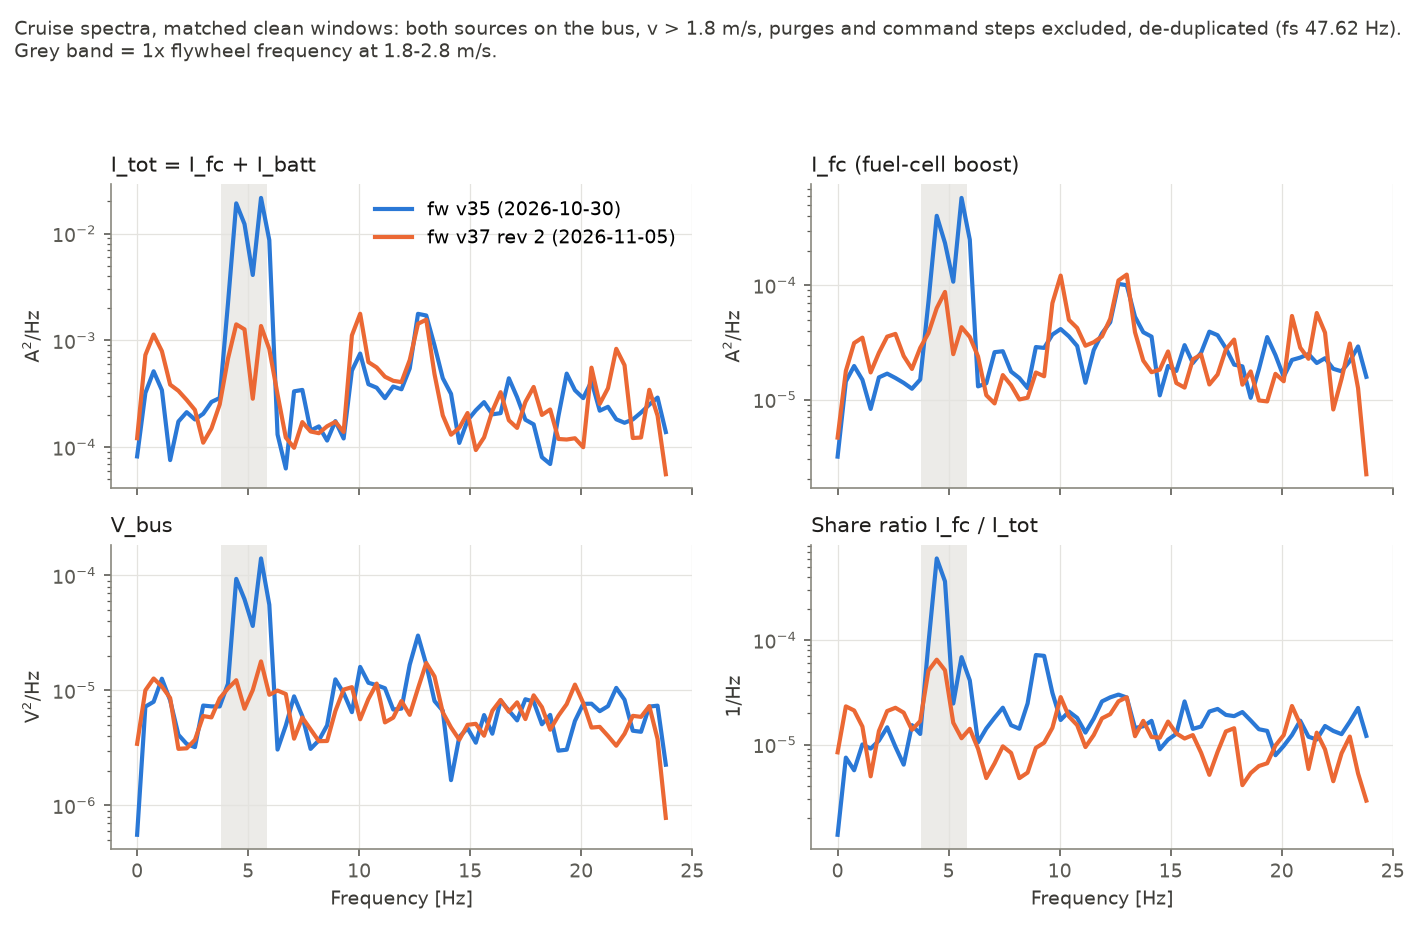
\includegraphics[width=0.86\linewidth]{brief_psd_before_after.png}\\
\textbf{Figure 1.} Cruise PSDs (v $>$ 1.8 m/s), fw v35 (blue) and fw v37 (orange). Grey band:
1x frequency at 1.8--2.8 m/s.
\end{center}

The share ratio appeared not to improve because two terms that the drive law does not touch
dominate it: the H-20 purges and the SDP command steps. Figure~2 shows the share 2--6~Hz rms as
each term is removed. With both removed, the share noise falls from 0.021 to 0.010.

\begin{center}
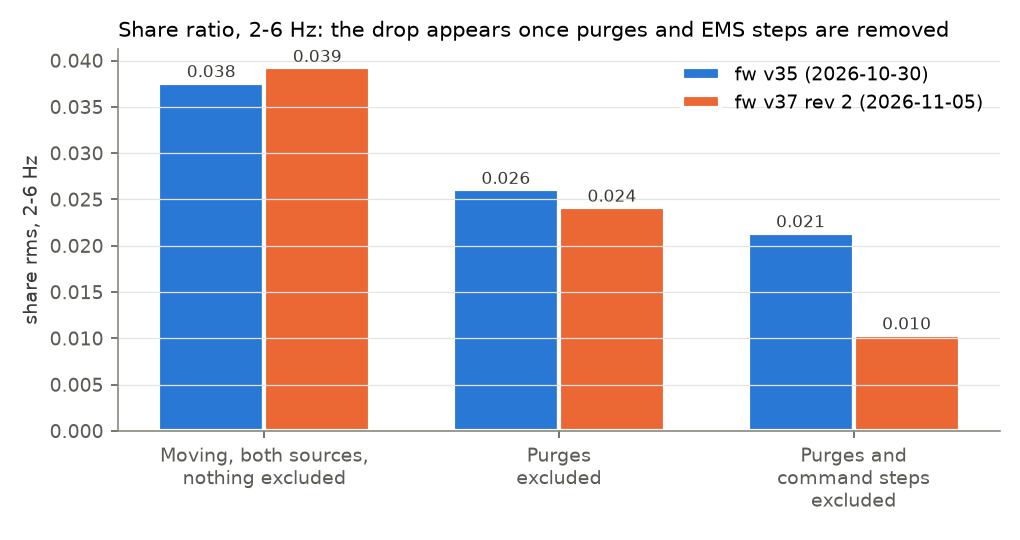
\includegraphics[width=0.48\linewidth]{brief_share_masks.png}\\
\textbf{Figure 2.} Share-ratio rms, 2--6 Hz, under successive masks.
\end{center}

Figure~3 breaks down the uncommanded share n = s $-$ cmd in the clean windows. The stacked areas
give the part of n that is coherent with the 1x rotation angle, then with \Itot, then with
V\textsubscript{fc}. In the 2--6~Hz band, the 1x-locked part falls from 0.018 to 0.007 rms. The
governor floor reference, 0.125~A / \Itot{} filtered over 19.5~ms, follows n closely in this band
(0.026 against 0.025 before, 0.011 against 0.011 after). The remaining 1x share term is therefore
the setpoint clip at the minority-current floor, which the share loop tracks; it is not a loop
deficiency. Above about 6~Hz both runs show a flat floor of about 0.011 rms, which Section~4
identifies as mostly folded content.

\begin{center}
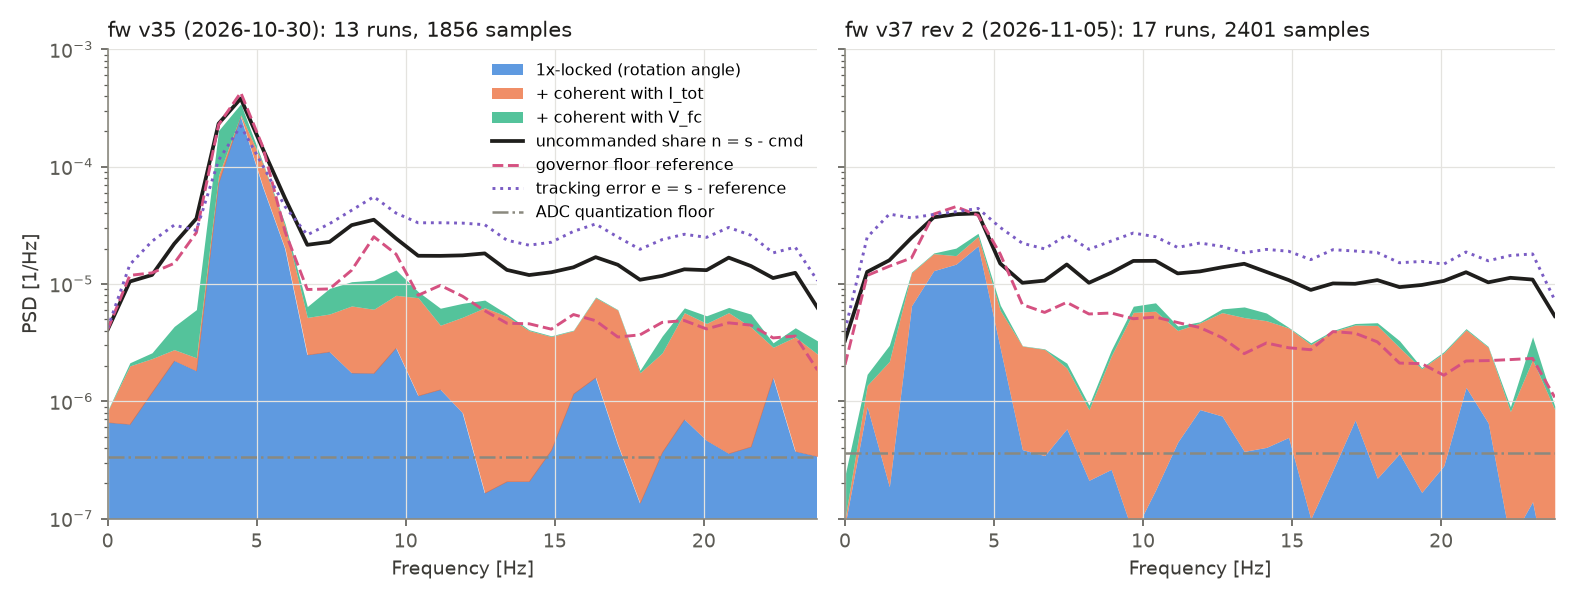
\includegraphics[width=\linewidth]{brief_share_budget.png}\\
\textbf{Figure 3.} Uncommanded share PSD and its coherent parts, clean windows (both sources on
the bus, v $>$ 0.3 m/s, purges and command steps excluded, de-duplicated).
\end{center}

\section*{4. Remaining \Vbus{} ripple: switching noise and the ideal diodes}
The bag cannot resolve anything above its 23.8~Hz Nyquist frequency. This section therefore uses a
1~kHz SD-card log, ML0226 (fw v37, bench). Its FC input is a bench supply (11.1~V, no purges), its
battery input is the pack, and it contains closed-loop speed holds at 1.0, 1.5 and 2.0~m/s. The
firmware loop and the log run at about 875~Hz (median tick 1131~$\mu$s), not 1~kHz.

Figure~4 shows the \Vbus{} spectrum at the loop rate and what a 21~ms telemetry snapshot makes of
it.

\begin{center}
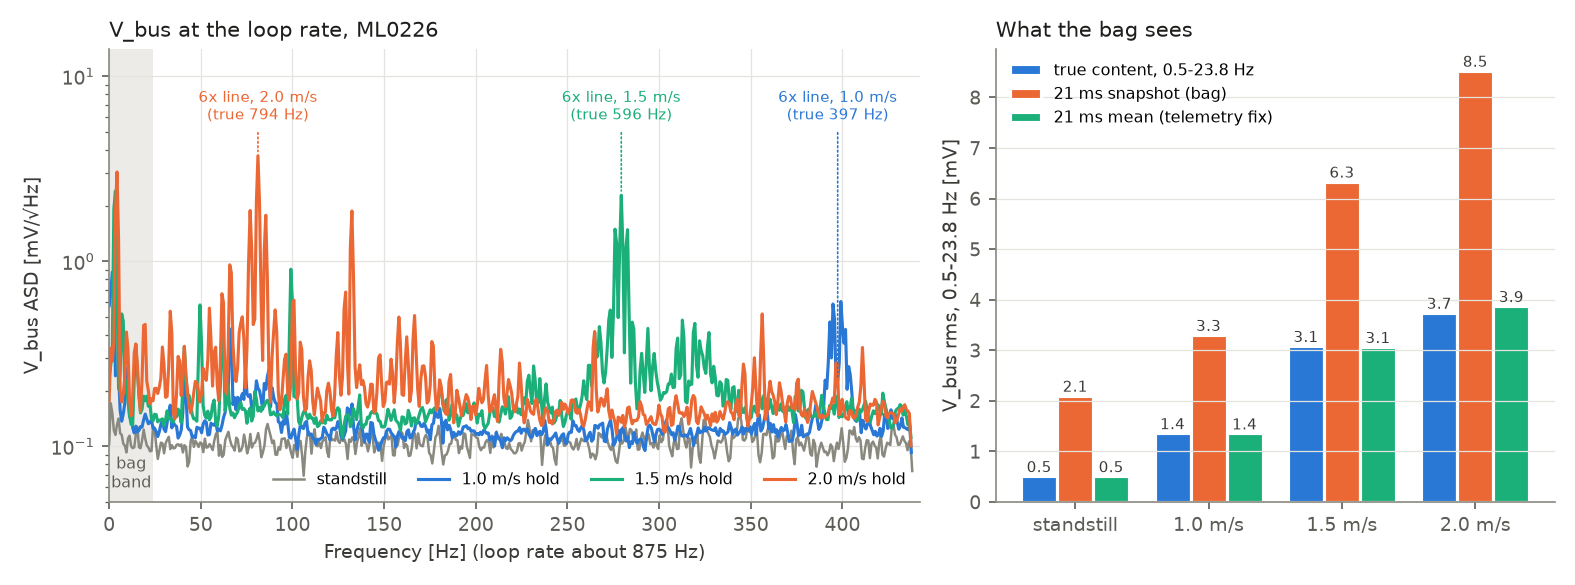
\includegraphics[width=\linewidth]{brief_vbus_1k.png}\\
\textbf{Figure 4.} Left: \Vbus{} amplitude spectral density in ML0226. The dotted markers show
where the motor 6x electrical line lands after folding at the loop's Nyquist frequency. Right:
\Vbus{} rms in 0.5--23.8~Hz for the true signal, a 21~ms snapshot and a 21~ms mean.
\end{center}

Three results follow from Figure~4:
\begin{itemize}\setlength{\itemsep}{0pt}
\item \textbf{Most of the bag's \Vbus{} noise is folded.} The snapshot reads 2.1--8.5~mV against
0.5--3.7~mV of true in-band content; 72--98\,\% of the snapshot variance comes from above
23.8~Hz. A 21~ms mean removes the fold almost completely.
\item \textbf{The standstill floor is the ADC chain.} At standstill, \Vbus, V\textsubscript{rgn},
I\textsubscript{fc} and I\textsubscript{batt} all read 0.42--0.50~LSB, with cross-channel
correlation of 0.06 or less.
\item \textbf{The dominant moving line is the motor's 6x electrical order.} It lies at 397~Hz per
m/s, which is 6 times the electrical frequency of the 2-pole-pair motor, so it is real at
600--1000~Hz at cruise. It is coherent with \Itot{} at 0.94--0.99 and with the commanded motor
current at only 0.01--0.05, so it is real current that the VESC draws from the bus. The bus
impedance at this line is 81--133~m$\Omega$, about 1.5 times its low-frequency value.
\end{itemize}

Table~3 gives the resulting budget for the bag at fw v37 cruise (about 12.6~mV rms per sample).
The split is measured on the bench and scaled to the vehicle; that scaling is not verified.

\begin{center}
\small
\begin{tabular}{lrl}
\toprule
Source & mV rms & Confidence \\
\midrule
Folded motor 6x electrical line and other speed-locked orders & 8--10 & Medium \\
Folded broadband excess (likely VESC 15~kHz PWM alias) & 5--6 & Low--medium \\
ADC floor, folded & 2.7--3.3 & High \\
Real 1x droop response to \Itot{} (2--6~Hz) & 2.4 & High \\
TPS61288 switching and PFM ripple, aliased & $\leq$ 1.2 & Medium \\
RT1987 ideal diodes & $\leq$ 0.6 & Medium--high \\
\bottomrule
\end{tabular}\\[0.3em]
\textbf{Table 3.} Budget of the \Vbus{} noise in the bag band, fw v37 cruise. The quadrature sum
of the central values is 12.3~mV.
\end{center}

\textbf{The RT1987 ideal diodes add no measurable \Vbus{} noise.} Below about 1.75~A, which covers
every current on the rig, each switch servos a forward drop of about 35~mV (RT1987 datasheet
p.7 and Section 17.6). The typical curve adds about 10~m$\Omega$ of incremental resistance. The
common 35~mV cancels in the share, so the switches are not the source of the estimated
$-$45 to $-$65~mV no-load mismatch between the sources; the TPS61288 reference tolerance can account
for it. No FC dropout or switch chatter occurs at the minority floor: no ML0226 sample with
\Itot{} above 0.2~A reads I\textsubscript{fc} below 4~mA, and every zero I\textsubscript{fc} in the
bags falls inside an H-20 purge. The servo bandwidth is not specified. Above it, each switch acts as
a resistance of about 35~mV / I, which filters boost ripple and is a candidate for the impedance
rise at 600--800~Hz. Neither effect has been measured.

\textbf{Boost switching contributes little to \Vbus.} The FC boost runs in light-load (PFM) mode
at all rig currents, and the battery boost runs near its PFM boundary of about 0.45~A. The PFM
ripple appears strongly on I\textsubscript{fc} (about 40~mA per sample) and V\textsubscript{fc},
because the shunt sits upstream of the ideal diode, but only weakly on \Vbus.

\textbf{Consequence for filtering.} A 20~ms mean in the telemetry would remove most of the folded
noise in the bags. However, the loop itself samples at 875--1000~Hz, so the 6x line folds near DC
in the control samples at about 2.2--2.5~m/s, the cruise speed. No digital filter after sampling
can remove that alias. Only an analog filter at the ADC pin, or averaging over the full loop
tick, prevents it.

\section*{5. Conclusions}
\begin{itemize}\setlength{\itemsep}{0pt}
\item The lower crossover reduced the 1x line to 0.25--0.28 on all bus channels and the share
ratio, in agreement with the design.
\item The share-ratio reduction is real. Purges and command steps hide it in unmasked data. The
remaining 1x share term is the governor's minority-current floor, not a loop deficiency.
\item \Vbus{} at 1x is the droop image of \Itot{} through about 70~m$\Omega$.
\item Most of the remaining \Vbus{} noise in the bags is folded high-frequency content. The largest
part is real bus current at the motor's 6x electrical frequency. The ideal diodes and the boost
switching contribute little.
\item Content above 7~Hz did not change with fw v37. A 20~ms telemetry mean removes most of it from
the bags. An analog filter at the ADC pins is needed to keep the 6x line out of the control
samples.
\item The tracking cost is visible: the speed-error rms below 0.7~Hz increased from 5.0 to
9.8~mm/s.
\item A vehicle 1~kHz SD-card log with the H-20 and the pack is needed to confirm the budget at
the vehicle operating point.
\end{itemize}

\end{document}
